\documentclass[tikz,border=10pt]{standalone}
% No extra TikZ libraries needed.
\begin{document}
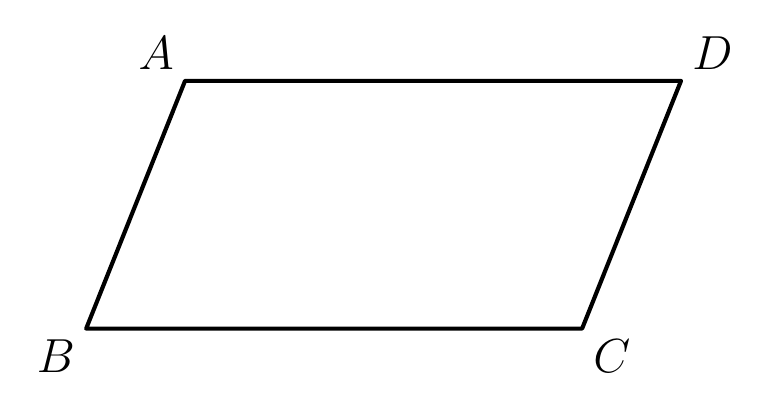
\begin{tikzpicture}[line join=round, line width=1.5pt]
  % Vertices: px -> units with s = 1/75 cm per px, centred on vertex bbox, y flipped
  \coordinate (A) at (-2.5242499999982178,1.572999999981679);
  \coordinate (B) at (-3.779750000001199,-1.5729999999877702);
  \coordinate (C) at (2.518749999998273,-1.572999999981674);
  \coordinate (D) at (3.7742500000011434,1.5729999999877646);

  % Trapezoid edges AB, BC, CD, DA (solid black)
  \draw[black] (A) -- (B) -- (C) -- (D) -- cycle;

  % Labels (17 pt font from style metrics)
  \node[above left,  font=\fontsize{17}{20.4}\selectfont] at (A) {$A$};
  \node[above right, font=\fontsize{17}{20.4}\selectfont] at (D) {$D$};
  \node[below left,  font=\fontsize{17}{20.4}\selectfont] at (B) {$B$};
  \node[below right, font=\fontsize{17}{20.4}\selectfont] at (C) {$C$};
\end{tikzpicture}
\end{document}